\chapter[Hierarchical Selective Classification of European Land Use / Land Cover using pixel-based uncertainty]{Hierarchical Selective Classification of European Land Use / Land Cover using pixel-based uncertainty}
\label{cha:chapter4}
\vspace*{\fill}
This chapter is based on:
\\
\\
% Full citation of the published (or submitted/in review) article
% This refers to the article key in the refs.bib file.
\fullcite{witjes2024hierarchical}
\newpage

\section*{Abstract}


\newpage

\section{Introduction}

\section{Methods}

\begin{figure}[H]
    \centering
    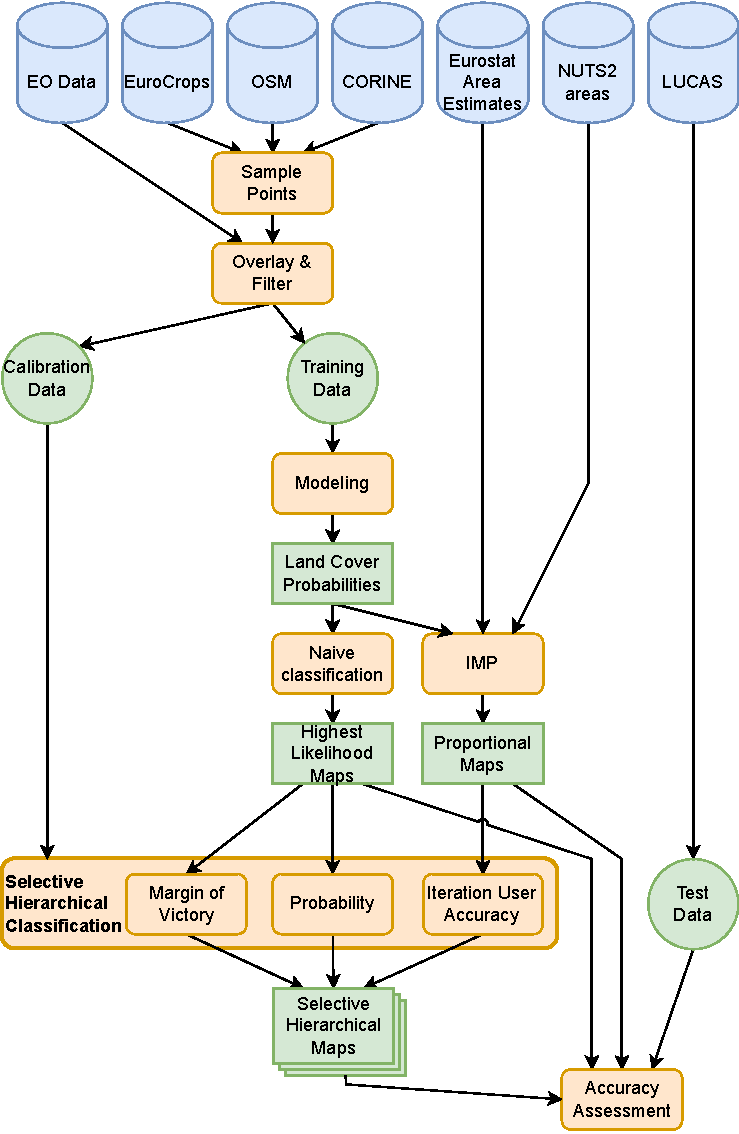
\includegraphics[width=\textwidth]{figs_05/fig_methodology.pdf}
    \caption{Caption}
    \label{fig:05_methodology}
\end{figure}

\subsection{Selection of study area}

We obtained Nomenclature of Territorial Units for Statistics (NUTS) administrative boundaries from EuroStat. %https://ec.europa.eu/eurostat/web/gisco/geodata/reference-data/administrative-units-statistical-units/nuts
We matched level 2 NUTS areas to the earliest LUCAS survey since each update (See Table~\ref{tab:05_NUTS_LUCAS}). 

We selected all NUTS2 areas:
1. For which LUCAS land cover area estimates were available;
2. For which more than 500 LUCAS points were available;
2. Whose area was below the largest 1\% surface area among NUTS2 areas (to maintain computational feasibility)

We randomly selected up to four NUTS2 area/year combinations each country.

\begin{table}[H]
    \centering
    \begin{tabular}{c|c}
         NUTS update year &  LUCAS survey year\\
         2006 & 2006 \\
         2010 & 2012 \\
         2013 & 2015 \\
         2016 & 2018 \\
    \end{tabular}
    \caption{Caption}
    \label{tab:05_NUTS_LUCAS}
\end{table}

\subsection{Legend harmonization}
% https://docs.google.com/spreadsheets/d/1UJrbdGJgrXlW_WnSoDVIhf68dz8XoiWrZW6WVeR5lPw/edit#gid=1654270911
For some classes, either no area estimates or no training data was available. This required us to exclude some classes, and aggregate others. The following classes were omitted completely:
\begin{itemize}
    \item B54: Mixed cereals for fodder
    \item E10: Grassland with sparse tree/shrub cover
    \item E30: Spontaneously re-vegetated surfaces
\end{itemize}
These classes were combined into 'Other' in the area estimates.

Lack of specific data on orange groves lead us to merge B76: Oranges with B77: Other citrus fruit`
Lastly, a number of level 3 classes were aggregated to their level 2 category. Table \ref{tab:05_legend_aggregation} shows an overview.

% Please add the following required packages to your document preamble:
% \usepackage{booktabs}
% \usepackage{multirow}
\begin{table}[]
\begin{tabular}{@{}ll@{}}

Level 3 LUCAS class & Aggregated LUCAS class \\ 
\midrule
A11: Buildings with one to three floors & A10: Roofed built-up areas \\
A12: Buildings with more than three floors &  \\
A21: Non built-up area features & \multirow{2}{*}{A20: Artificial non-built up areas} \\
A22: Non built-up linear features &  \\
C21: Spruce dominated coniferous woodland & \multirow{3}{*}{C20: Coniferous woodland} \\
C22: Pine dominated coniferous woodland &  \\
C23: Other coniferous woodland &  \\
C31: Spruce dominated mixed woodland & \multirow{3}{*}{C30: Mixed woodland} \\
C32: Pine dominated mixed woodland &  \\
C33: Other mixed woodland &  \\
G11: Inland fresh water bodies & \multirow{2}{*}{G00: Water} \\
G12: Inland salty water bodies &  \\
G21: Inland fresh running water &  \\
G22: Inland salty running water &  \\
\midrule
\end{tabular}
\caption{Overview of which original LUCAS level 3 classes were aggregated to }
\label{tab:05_legend_aggregation}
\end{table}

\subsection{Training Data}
We extracted polygons from CORINE, EuroCrops and OpenStreetmap. Table~\ref{tab:05_sources} shows the training data source per LUCAS class.

We randomly sampled points from polygons.

We filtered the training data



\subsection{Validation Data}

\section{Results}
\subsection{Training data}
\subsection{Validation data}

Sampling up to four NUTS2 area/year combinations with more than 500 LUCAS points and available area estimates resulted in 93 selected areas. Figure~\ref{fig:05_lucas_aoi} shows the selected areas and gives an overview of the level 1 land cover classes of the LUCAS points they contain. Figure~\ref{fig:05_lucas_aoi_counts} shows the number of validation points per class across all areas.

\begin{figure}[h]
    \centering
    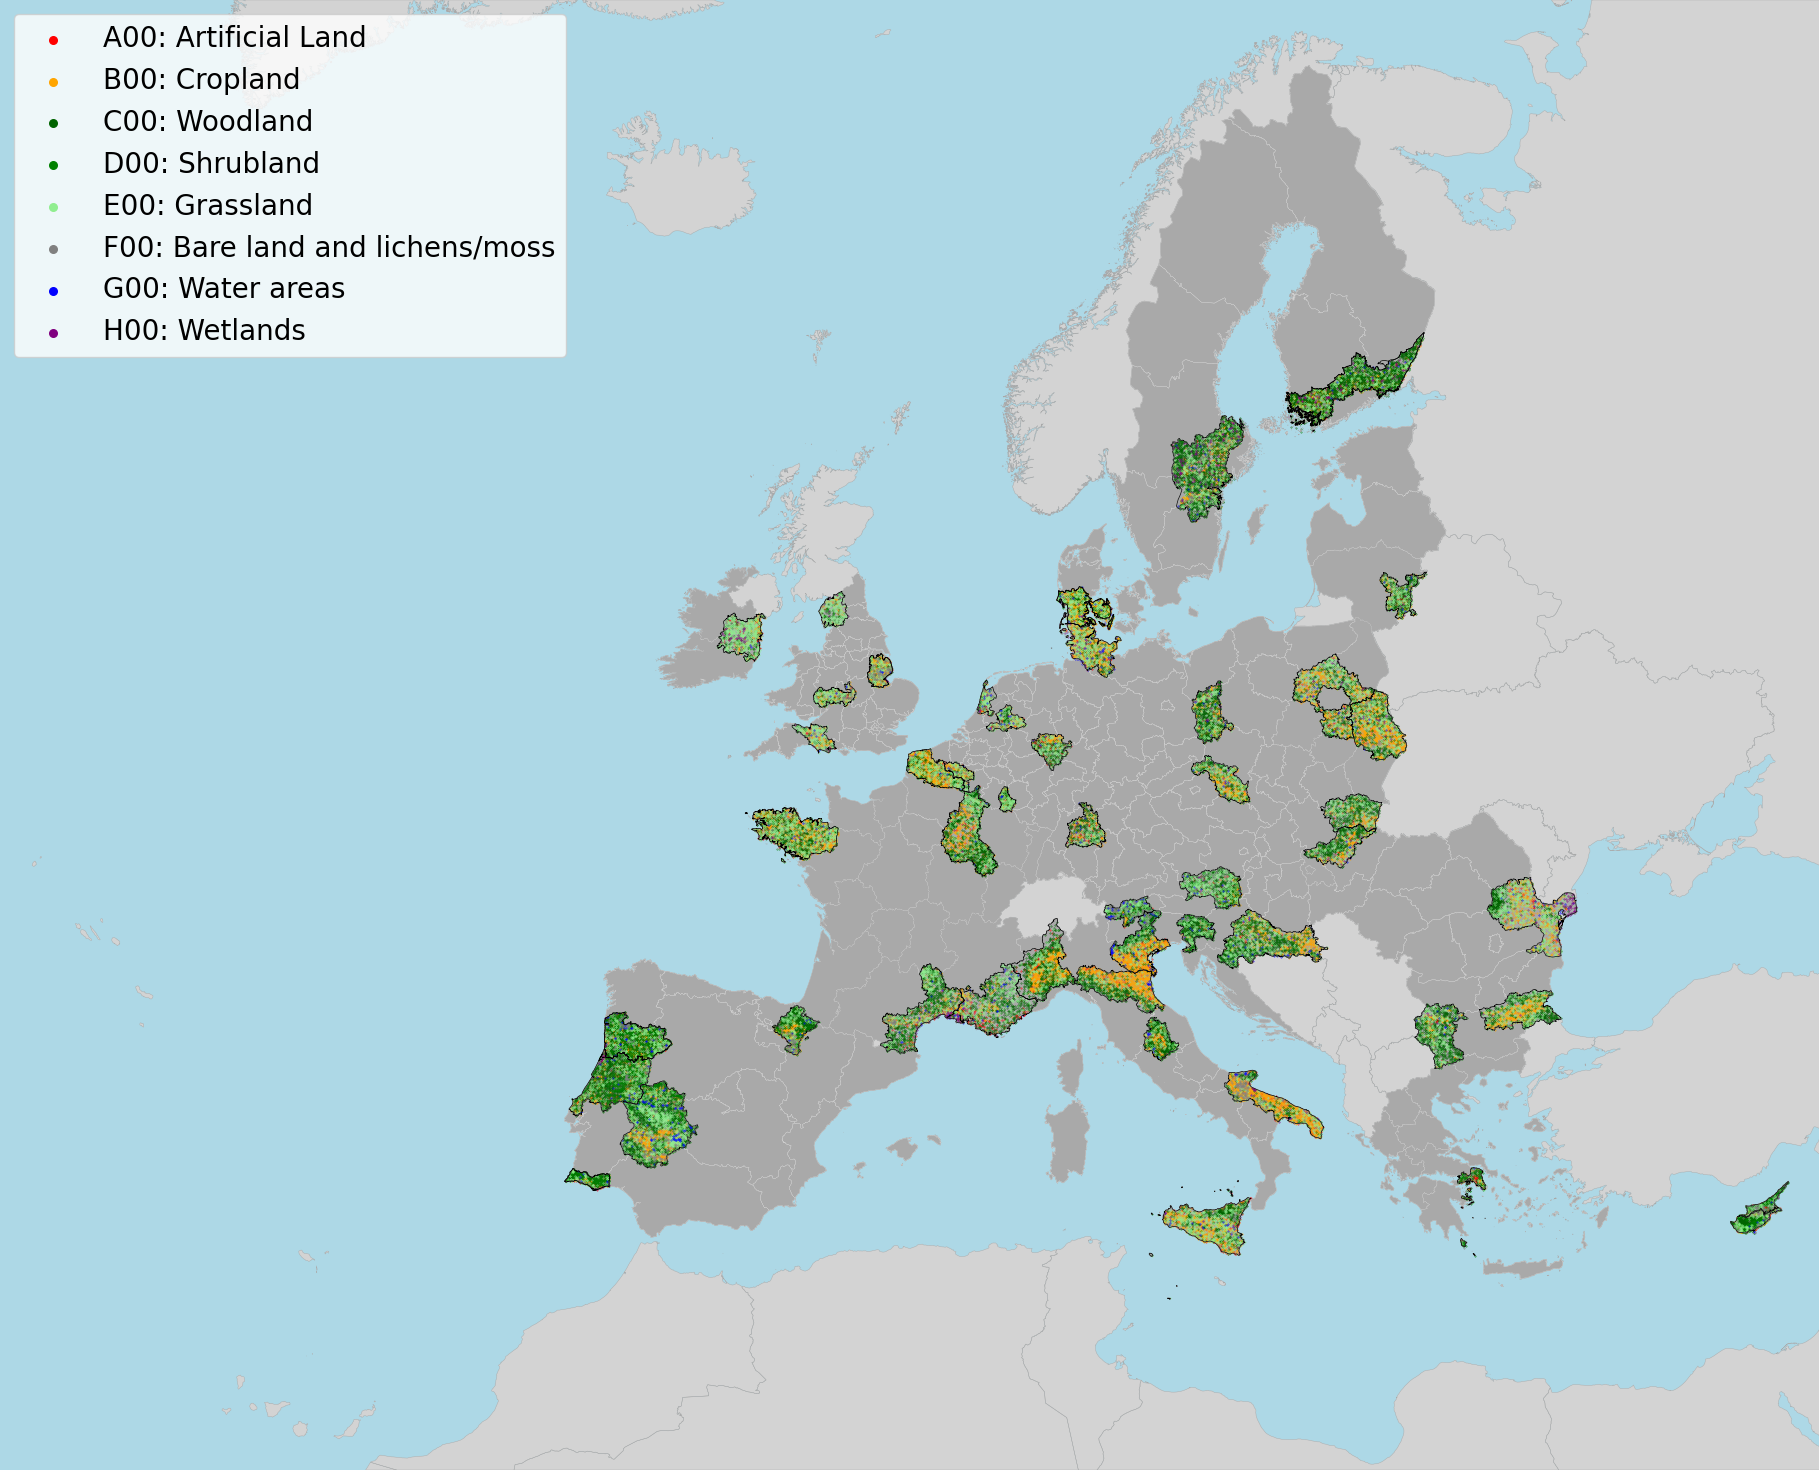
\includegraphics[width=\textwidth]{figs_05/fig_lucas_aoi.png}
    \caption{LUCAS points in sampled NUTS2 areas, used for validation of all land cover maps}
    \label{fig:05_lucas_aoi}
\end{figure}

\begin{figure}[h]
    \centering
    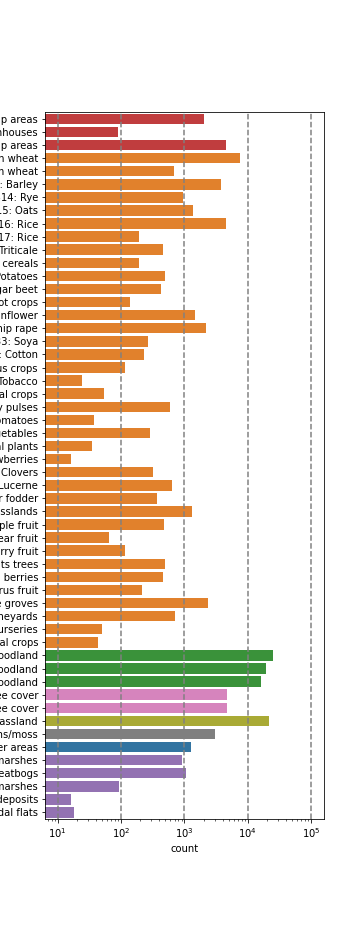
\includegraphics[width=\textwidth]{figs_05/fig_lucas_aoi_counts.png}
    \caption{Number of LUCAS points per LUCAS class used to validate theland cover maps, colored based on their level 1 class.}
    \label{fig:05_lucas_aoi_counts}
\end{figure}

\section{Discussion}

    \subsection{Legend}
        We lost a lot of detail in our legend because we needed 1) training data, 2) area estimates, and 3) validation points. We had training data for a lot of water \& bare land subclasses. It would be good if Eurostat made area estimates for all LUCAS land cover classes; we could have included them.